% Compile on Overleaf with pdfLaTeX; main document: main.tex.
% Uses the official Springer Nature journal class (December 2024 package).
\documentclass[pdflatex,sn-mathphys-num]{sn-jnl}
\usepackage{graphicx,amsmath,amssymb,booktabs,tabularx,array}
\usepackage{tikz,pgfplots}
\usetikzlibrary{arrows.meta,positioning}
\usepgfplotslibrary{groupplots}
\pgfplotsset{compat=1.18}
\usepackage{placeins}
\hypersetup{hidelinks,pdftitle={DriveAlert AI Case Study Report},pdfauthor={Krishnan S, Adwaith Raveendran, Eric Febin}}
\newcolumntype{Y}{>{\raggedright\arraybackslash}X}
\let\burl\url
\raggedbottom

\begin{document}

\title[DriveAlert AI]{DriveAlert AI for Context Aware Driver Fatigue and Microsleep Monitoring}
\author[1]{\fnm{Krishnan} \sur{S}}
\author[1]{\fnm{Adwaith} \sur{Raveendran}}
\author[1]{\fnm{Eric} \sur{Febin}}
\affil[1]{\orgdiv{Department of Computer Science and Engineering}, \orgname{Amrita Vishwa Vidyapeetham}, \orgaddress{\country{India}}}

\abstract{DriveAlert AI is a webcam-based research prototype that combines eye-state and mouth-event classification with temporal fatigue rules and simulated driving context. This case study examines its current implementation, model evaluation and integration limits. Separate MobileNetV3-Small classifiers process eye and mouth crops, while a deterministic engine combines sustained closure, a PERCLOS proxy and repeated yawns. Simulated speed and continuous-drive duration change temporal alert sensitivity. A React interface displays evidence, speaks predefined warnings and offers a demonstration rest route. MobileNetV3-Small, EfficientNet-B0 and ResNet-18 were evaluated using participant-disjoint crop splits and validation-selected operating thresholds. The deployed MobileNet models achieved 96.93\% eye balanced accuracy and 94.41\% mouth balanced accuracy against provisional weak labels. ResNet-18 achieved higher balanced accuracy at substantially greater parameter and computation cost. A saved CPU benchmark measured 94.31 ms median for the MobileNet pair and normalization, excluding the camera and service pipeline. Integration checks identified a 700 ms browser sampling interval that exceeds the engine's 500 ms continuity allowance, preventing sustained-closure accumulation at that cadence. The work demonstrates component integration and a controlled model comparison; reliable event detection requires timing correction, independent annotation and end-to-end evaluation under representative driving conditions.}

\keywords{Driver fatigue, microsleep monitoring, MobileNetV3, eye state classification, PERCLOS, temporal decision rules}
\maketitle
\raggedbottom
\clearpage

\section{Introduction}\label{sec:introduction}
Driver fatigue monitoring requires more than recognising an isolated closed eye or an open mouth. A brief blink may be normal, a mouth movement may be speech, and an unavailable camera signal should not be interpreted as evidence that a driver is alert. A practical monitoring system must connect visual observations to their duration, distinguish valid evidence from missing observations, and communicate a useful response. These requirements motivate DriveAlert AI, a college research prototype intended to explore affordable monitoring with a standard RGB camera.

The application focuses on commercial-transport use cases in which long or irregular driving schedules motivate timely rest advice. Its present operating environment is a local computer and a browser. A camera provides facial images, but vehicle speed and continuous-drive duration are entered through examiner controls. The displayed route to a rest plaza is predefined. The implemented scope therefore supports a laboratory demonstration of monitoring and intervention; it does not establish accident reduction, vehicle integration or validated on-road safety.

The project addresses two linked questions. First, what classification and computational trade-offs arise when MobileNetV3-Small, EfficientNet-B0 and ResNet-18 use a shared eye-and-mouth evaluation protocol? Second, how can compact visual classifiers feed a transparent temporal policy whose alert sensitivity depends on driving context? The first question is supported by saved evaluation results. The second is implemented as an engineering policy, but its effect on detection delay and false alarms has not yet been established experimentally.

We use two separately trained models: one predicts open or closed eye state, and the other distinguishes non-yawning, talking and yawning. Their probabilities feed a deterministic engine that accumulates evidence over time. This separation makes model outputs, temporal thresholds and alert reasons visible in the interface and independently testable. It also exposes integration requirements: successful frame classification does not guarantee that the observation cadence is suitable for detecting short events.

The contribution of this case study is a documented prototype combining participant-disjoint model comparison, locked operating thresholds, explicit temporal evidence, simulated speed and drive-time sensitivity, and a rest-oriented interface. The backbones are established architectures, and adaptive temporal warning already appears in prior work. Accordingly, the project claims an implementation and evaluation framework rather than a new neural architecture or demonstrated superiority over commercial driver-monitoring systems.

\section{Related Work}\label{sec:related}
\subsection{Lightweight classification and deployment}
MobileNetV3 uses architecture search and mobile-oriented building blocks to reduce computation, EfficientNet studies balanced scaling of network dimensions, and ResNet introduces residual learning to support deeper networks \cite{howard2019mobilenetv3,tan2019efficientnet,he2016resnet}. These architectures motivate the three alternatives evaluated here. Their original ImageNet results do not establish performance on the project's fatigue-related tasks; task-specific training and held-out testing remain necessary.

Vimala et al. investigate lightweight deep learning for driver fatigue detection and compare MobileNet and EfficientNet variants \cite{vimala2026lightweight}. This is the project's selected application reference because it links model selection to deployment cost. Bhanja et al. describe an eye-based MobileNet webcam system \cite{bhanja2025ddsh}, while Choi et al. study event-driven blink tracking with specialised hardware \cite{choi2025ebts}. Together, these approaches show why sensor choice, computation and the alert pipeline must be considered alongside classifier performance. DriveAlert uses ordinary RGB capture and a local CPU service; it has not measured energy use or compared directly with event-camera hardware.

\subsection{Temporal representation and driver variation}
Wei et al. model several sources of prior-informed facial information using graph convolution \cite{wei2025migcn}. Qin et al. use landmark heatmaps and spatial-temporal attention for video-based detection \cite{qin2025heatmaps}. Kim et al. address calibration-free cross-subject classification using EEG and prototype-based multi-domain mixup \cite{kim2025calibration}. Although their sensors and representations differ, these studies motivate temporal reasoning and explicit treatment of participant identity. DriveAlert uses recorded participant identifiers to separate training, validation and test crops. It does not reproduce their tasks or claim that one crop hold-out experiment establishes cross-domain generalisation.

Hybrid visual representations provide another comparison. EffRes-DrowsyNet combines EfficientNetB0 and ResNet50 \cite{algburi2025effres}; Xu et al. study hybrid facial features and ensemble learning \cite{xu2025hybrid}; and Abd El-Nabi et al. investigate attention-enhanced convolutional monitoring \cite{elnabi2026attention}. The DriveAlert comparison instead evaluates three standalone backbones under aligned settings. Evidence for ResNet50 or a hybrid model cannot be treated as a direct result for ResNet-18.

\subsection{Robustness and intervention}
Liu et al. investigate fatigue detection under complex lighting \cite{liu2025yolofdcl}. Xie and Xiao use confidence-driven adaptive observation windows with temporal modelling \cite{xie2026adaptive}. Their work makes clear that adaptive timing is not unique to this project. A relevant future experiment is to compare fixed, confidence-adaptive and speed-and-duration-adaptive policies using the same independently annotated event sequences.

Broader systems research considers multimodal state estimation and interpretability \cite{sah2026multimodal}, as well as drowsiness alerts and accident-prevention applications \cite{mahapatra2026alerts}. Reviews by Hassan et al. and Rabbi et al. organise monitoring technologies and CNN approaches \cite{hassan2026survey,rabbi2026review}. These works motivate a system-level perspective, but reported accuracy values across different datasets, labels and split protocols should not be ranked as one common benchmark. This report therefore compares only the project's three models numerically and treats the literature as methodological context.

\section{Methodology}\label{sec:method}
\subsection{System architecture and current workflow}
Figure~\ref{fig:architecture} shows the implemented pipeline. The React 18 and Vite interface acquires a camera stream after browser permission, resizes transmitted frames to 640 pixels in width and encodes JPEG images at quality 0.72. It schedules one analysis request every 700 ms and suppresses overlapping requests. The nominal request frequency is approximately 1.43 Hz; this is distinct from webcam frame rate and processing latency.

The local Python service uses \texttt{ThreadingHTTPServer}. Its status endpoint reports model and extraction information, its analysis endpoint accepts a frame with a session identifier and telemetry, and its reset endpoint clears session history. The analysis response returns facial-region boxes, classifier probabilities, temporal metrics, effective thresholds, alert reasons and processing time. Each session maintains its own fatigue engine. Evidence timestamps come from the server's monotonic clock after prediction rather than from camera acquisition.

\begin{figure}[htbp]
\centering
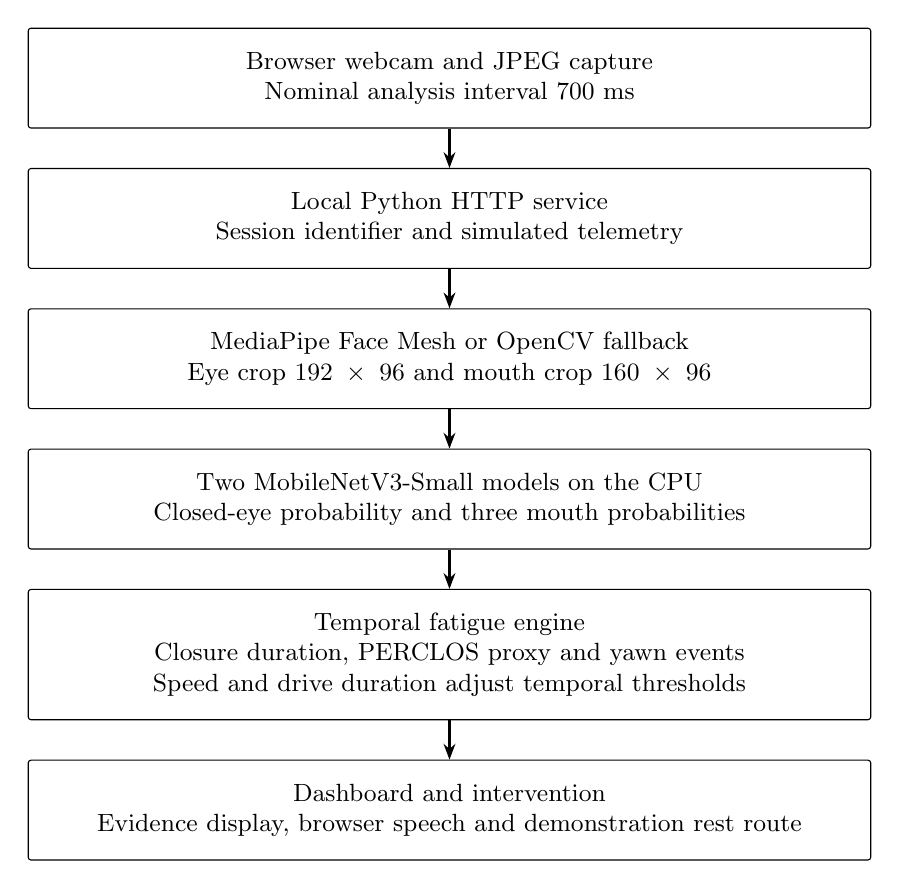
\begin{tikzpicture}[node distance=5mm,box/.style={draw,rounded corners=1pt,align=center,font=\small,text width=10.1cm,minimum height=8mm,inner sep=3mm},arr/.style={-{Stealth[length=2mm]},thick}]
\node[box] (camera) {Browser webcam and JPEG capture\\Nominal analysis interval 700 ms};
\node[box,below=of camera] (api) {Local Python HTTP service\\Session identifier and simulated telemetry};
\node[box,below=of api] (vision) {MediaPipe Face Mesh or OpenCV fallback\\Eye crop $192\times96$ and mouth crop $160\times96$};
\node[box,below=of vision] (models) {Two MobileNetV3-Small models on the CPU\\Closed-eye probability and three mouth probabilities};
\node[box,below=of models] (engine) {Temporal fatigue engine\\Closure duration, PERCLOS proxy and yawn events\\Speed and drive duration adjust temporal thresholds};
\node[box,below=of engine] (ui) {Dashboard and intervention\\Evidence display, browser speech and demonstration rest route};
\foreach \a/\b in {camera/api,api/vision,vision/models,models/engine,engine/ui}\draw[arr] (\a)--(\b);
\end{tikzpicture}
\caption{Implemented processing flow. EfficientNet-B0 and ResNet-18 are evaluated offline and are not loaded by the live service. Telemetry and routing are simulated.}\label{fig:architecture}
\end{figure}

\subsection{Datasets and provisional labels}
The data workflow uses UTA Real-Life Drowsiness Dataset (UTA-RLDD) and the Yawning Detection Dataset (YawDD), with attribution to their original publications \cite{ghoddoosian2019rldd,abtahi2014yawdd}. The eye task includes crops from both datasets, while the mouth splits contain YawDD crops. The project's task-specific crop labels and hold-out protocol differ from the datasets' original video-level evaluation settings.

The local extraction record contains 500 processed videos from 150 recorded participants: 180 UTA-RLDD videos and 320 YawDD videos. These are counts for the project corpus, not a claim about the complete source datasets. The preprocessing workflow extracts facial features and image crops, creates a manual-review queue, generates provisional weak labels, forms participant-disjoint splits and packages the processed data for notebook training. Eye and mouth aspect ratios (EAR and MAR), video information and quality indicators support this workflow. The existence of an annotation interface does not establish that all evaluation samples have independent human labels. All six saved model evaluations explicitly mark the labels as non-ground-truth and the models as provisional.

Weak eye labels use a three-sample rolling median and a per-video 80th-percentile EAR baseline clipped to $[0.22,0.42]$. A closed label requires an EAR-to-baseline ratio at most 0.60 and raw mean EAR at most 0.20; an open label requires a ratio at least 0.82 and raw EAR at least 0.21. Quality checks reject dark, blurred or asymmetric observations. Weak mouth labels combine source-video tags with a three-sample MAR median: normal clips require MAR at most 0.08, talking clips require MAR between 0.08 and 0.40, and yawning clips require MAR at least the larger of 0.25 and the video's 80th percentile. Ambiguous and mixed talking-yawning samples are excluded. These offline rules use temporal and video-level statistics and do not provide independently annotated online event boundaries. Participant splits use seed 20260829 and approximately 70/15/15 proportions within each dataset.

Table~\ref{tab:splits} reports the actual crop counts. The eye test set contains only 186 closed-eye examples among 3,918 crops, making accuracy alone an incomplete summary. Participant separation was checked using recorded dataset and person identifiers; the intersections across train, validation and test sets were zero for each task. This reduces identity leakage within the recorded splits but does not verify identity metadata, remove weak-label errors or make adjacent frames statistically independent.

\begin{table}[htbp]
\caption{Participant-disjoint task splits and class counts. Parentheses in the final column give the class order.}\label{tab:splits}
\begin{tabularx}{\textwidth}{@{}llrrY@{}}
\toprule
Task & Split & Crops & People & Class counts \\
\midrule
Eye & Train & 16,940 & 104 & 16,134 / 806 \\
& Validation & 3,572 & 23 & 3,293 / 279 \\
& Test & 3,918 & 23 & 3,732 / 186 (open / closed) \\
\midrule
Mouth & Train & 12,023 & 62 & 6,434 / 4,403 / 1,186 \\
& Validation & 2,884 & 14 & 1,475 / 1,105 / 304 \\
& Test & 2,847 & 14 & 1,633 / 935 / 279 (non-yawn / talking / yawn) \\
\bottomrule
\end{tabularx}
\end{table}

\subsection{Region extraction and input preparation}
The primary extractor uses MediaPipe Face Mesh with one face, refined landmarks, and detection and tracking confidence settings of 0.60. Eye contours from both eyes form one combined region; the mouth contour forms the other. Each region receives geometric padding, is clipped to image boundaries and is resized while preserving aspect ratio. Letterboxing uses the median colour of the resized crop. This reduces geometric distortion but is not a learned denoising method.

If MediaPipe initialisation raises a runtime error, the implementation can use an OpenCV Haar-cascade detector and approximate eye and mouth locations within the largest detected face. This fallback offers continuity of the demonstration, but its crop quality has not been separately validated. The landmark route also computes EAR and MAR as diagnostic values. The live fatigue decision uses neural probabilities rather than direct EAR or MAR thresholds.

Input crops are converted from BGR to RGB, scaled to $[0,1]$, normalised using ImageNet channel means $(0.485,0.456,0.406)$ and standard deviations $(0.229,0.224,0.225)$, and arranged as channel-first tensors. Eye images have width 192 and height 96; mouth images have width 160 and height 96. The training transformations include horizontal flipping, colour jitter and a small affine transformation. Gaussian-noise injection, a motion-blur training kernel, random erasing and an explicit moving-average landmark filter are not part of the inspected implementation. Robustness to night conditions, eyewear and camera vibration remains an evaluation requirement.

\subsection{Neural architectures and training}
MobileNetV3-Small, EfficientNet-B0 and ResNet-18 use ImageNet-pretrained backbones with task-specific output layers. Each architecture has a one-logit eye classifier and a three-logit mouth classifier. MobileNetV3-Small uses depthwise processing, inverted residual blocks and squeeze-and-excitation components; EfficientNet-B0 uses mobile inverted bottlenecks; ResNet-18 uses residual blocks. These are alternative models, not a three-model ensemble.

For an eye logit $z_e$, the model produces $p_e=\sigma(z_e)$. For mouth logits $\mathbf{z}_m$, softmax produces the probabilities of non-yawning, talking and yawning. The live eye label is closed when $p_e\geq0.060$. A mouth observation is labelled yawn when its yawn probability is at least 0.355; otherwise, the larger of the non-yawn and talking probabilities determines the label.

Class imbalance is handled during training. The eye loss is binary cross-entropy with positive-class weight
\begin{equation}
 w_+=\sqrt{N_{\mathrm{open}}/N_{\mathrm{closed}}}
     =\sqrt{16134/806}\approx4.47.
\end{equation}
The mouth loss uses cross-entropy with normalised inverse-square-root class-frequency weights and label smoothing of 0.03. This weighting gives rare classes more influence without using the full inverse-frequency ratio. Table~\ref{tab:training} summarises shared optimisation settings.

\begin{table}[htbp]
\caption{Training and operating-point configuration.}\label{tab:training}
\begin{tabularx}{\textwidth}{@{}p{4.2cm}Y@{}}
\toprule
Setting & Configuration \\
\midrule
Initialisation & ImageNet-pretrained backbone, task-specific classifier \\
Optimiser & AdamW; weight decay $10^{-4}$ \\
Learning rates & Backbone $3\times10^{-5}$; classifier $3\times10^{-4}$ \\
Batch size and epoch cap & 128 for training, 256 for evaluation; maximum 15 epochs \\
Checkpoint selection & Validation AP for eye; validation macro AP for mouth \\
Early stopping & Four epochs without improvement \\
Scheduling & ReduceLROnPlateau; factor 0.5, patience 1, minimum $10^{-6}$ \\
Eye operating point & Maximise specificity subject to validation closed-eye recall $\geq90\%$ \\
Mouth operating point & Maximise non-yawn specificity subject to validation yawn recall $\geq90\%$ \\
Test use & Evaluate after checkpoint and probability threshold selection \\
\bottomrule
\end{tabularx}
\end{table}

Validation selects the checkpoint before searching for the operating threshold. The selected threshold is then locked for the held-out test set. The target of at least 90\% recall applies to validation and is not a guarantee about test recall. The deployed MobileNet checkpoints were selected at epoch 9 for the eye task and epoch 12 for the mouth task. The stored histories and metrics support retrospective inspection of this selection.

\subsection{Temporal evidence and sensor validity}
An isolated closed-eye label is insufficient for a fatigue alert. The temporal engine maintains continuous closure duration, a rolling PERCLOS proxy and a yawn-event history. It records at most 0.5 s for each gap between observations. A gap greater than 0.5 s restarts the continuous-closure timer. Let $\Delta_i$ be a recorded valid-eye interval, and let $c_i$ indicate that the previous valid observation was classified as closed. Each interval is capped at 0.5 s and clipped to the trailing window. Within a trailing 60 s window, the proxy is
\begin{equation}
 P_{60}=\frac{\sum_i\Delta_i c_i}{\sum_i\Delta_i}.
\end{equation}
The proxy is defined as zero when no valid duration exists. This classifier-based proportion requires independent validation against annotated eye closure before being interpreted as a validated PERCLOS measurement. The PERCLOS rules require at least 20 s of elapsed observation and valid-eye coverage of at least 60\% of the elapsed window. The window is 60 s, not 20 s; 20 s is the initial readiness requirement.

A yawn candidate starts when the yawn probability reaches 0.355 and counts on a qualifying observation at least 0.75 s later. Values below $0.355\times0.65$ or missing mouth evidence release the candidate. A 2 s cooldown and an active-event flag limit duplicate counting. Events are counted over 300 s. On each received observation, the engine returns sensor unavailable if no valid eye sample exists or the last valid sample is more than 2 s old. No independent timeout runs when requests stop. The current yawn candidate logic does not impose the eye pathway's maximum-gap reset, which warrants testing under irregular sampling.

\subsection{Speed and drive-duration adaptation}
Driving context changes the temporal policy while keeping the neural probability thresholds fixed. For speed $v$ in km/h and driving duration $h$ in hours, the combined sensitivity is $S=S_vS_h$, where
\begin{align}
S_v&=1+0.35\min\!\left(1,\max\!\left(0,\frac{v-5}{95}\right)\right),\\
S_h&=\begin{cases}
1.00,&h<2,\\
1.10,&2\leq h<4,\\
1.25,&4\leq h<8,\\
1.40,&h\geq8.
\end{cases}
\end{align}
The maximum combined multiplier is 1.89. The base closure warning and critical thresholds are 1.50 s and 2.50 s; both are divided by $S$. The PERCLOS thresholds become $\max(0.08,0.15/S)$ and $\max(0.15,0.25/S)$. The repeated-yawn advisory threshold is $\max(2,\lceil3/S\rceil)$. These values are engineering defaults to be calibrated, not validated medical or regulatory thresholds.

For example, at 100 km/h and eight hours, $S=1.89$, giving closure thresholds of approximately 0.79 s and 1.32 s. PERCLOS thresholds reach their floors of 0.08 and 0.15, while two yawn events suffice for an advisory. At or above 5 km/h the engine applies its moving-vehicle severity logic. The browser separately pauses inference and resets evidence at exactly zero speed. These are distinct behaviours.

The highest applicable severity determines the result: monitoring, advisory, warning or critical, with sensor unavailable handled separately. Warning and critical states activate the intervention interface, subject to a 12 s modal throttle. Browser SpeechSynthesis reads predefined warnings after the user enables voice alerts. Accepting a rest recommendation activates a fixed route to Lakeside Rest Plaza. The interface contains no generative dialogue, live map search, GPS route computation or vehicle-control function.

\subsection{Evaluation measures}
We evaluate eye performance using average precision (AP), ROC-AUC, balanced accuracy, closed-eye precision and recall. If TP, FP, TN and FN denote the binary confusion counts, then
\begin{align}
\mathrm{Precision}&=\frac{\mathrm{TP}}{\mathrm{TP}+\mathrm{FP}},\qquad
\mathrm{Recall}=\frac{\mathrm{TP}}{\mathrm{TP}+\mathrm{FN}},\\*
\mathrm{Balanced\ accuracy}&=\tfrac12\!\left(\frac{\mathrm{TP}}{\mathrm{TP}+\mathrm{FN}}+
\frac{\mathrm{TN}}{\mathrm{TN}+\mathrm{FP}}\right).
\end{align}
For the mouth task, balanced accuracy is the mean of the three class recalls, macro F1 is the mean class F1, and macro AP is the mean one-versus-rest AP. Class-wise metrics distinguish yawning errors from talking errors. AP and ROC-AUC summarise rankings across thresholds, whereas the confusion matrices describe the selected operating point.

Computational evidence includes parameter counts and convolution/linear multiply-accumulate operations (MACs) at the actual crop sizes. One MAC is one multiply-accumulate, not a universally defined FLOP count. FP32 parameter storage is $4P$ bytes for $P$ parameters; it excludes activations and runtime overhead. Timing and unit checks are reported separately from classification performance.

\FloatBarrier
\section{Results and Discussion}\label{sec:results}
\subsection{Held-out classification performance}
Tables~\ref{tab:eye-results} and \ref{tab:mouth-results} report the saved test metrics against provisional weak labels. The three architectures use the same task split definitions. Their operating points are selected separately on validation. ResNet-18 has the highest eye balanced accuracy and mouth balanced accuracy in this comparison, while MobileNetV3-Small gives a smaller deployed model with a modest score reduction.

% Metric tables are generated directly from the saved evaluation JSON files.
\begin{table}[htbp]
\caption{Eye test results in percent on 3,918 crops. BA is balanced accuracy; precision and recall refer to closed eyes.}\label{tab:eye-results}
\begin{tabularx}{\textwidth}{@{}Yrrrrr@{}}
\toprule
Architecture & AP & AUC & BA & Precision & Recall \\
\midrule
MobileNetV3-Small & 94.14 & 99.51 & 96.93 & 58.39 & 97.31 \\
EfficientNet-B0 & 96.62 & 99.58 & 96.53 & 47.91 & 98.39 \\
ResNet-18 & 96.41 & 99.62 & 97.88 & 65.12 & 98.39 \\
\bottomrule
\end{tabularx}
\end{table}

\begin{table}[htbp]
\caption{Mouth test results in percent on 2,847 crops. BA averages the three class recalls; precision and recall refer to yawns.}\label{tab:mouth-results}
\begin{tabularx}{\textwidth}{@{}Yrrrrr@{}}
\toprule
Architecture & Macro AP & Macro F1 & BA & Precision & Recall \\
\midrule
MobileNetV3-Small & 98.33 & 95.02 & 94.41 & 96.95 & 91.04 \\
EfficientNet-B0 & 98.37 & 94.95 & 94.07 & 98.41 & 88.89 \\
ResNet-18 & 98.70 & 96.06 & 95.57 & 98.86 & 93.55 \\
\bottomrule
\end{tabularx}
\end{table}


The MobileNet eye model detects 181 of 186 closed-eye crops and misses five. It also classifies 129 open-eye crops as closed, yielding 58.39\% positive precision despite 97.31\% closed-eye recall. This is a material operating-point trade-off. The model's 96.93\% balanced accuracy must not be described as event-detection accuracy or as evidence of few driving-session false alarms. Temporal filtering may change the alert rate, but that effect needs sequence-level measurement.

For the mouth model, 254 of 279 yawns are recognised, while 25 are assigned to talking. Eight talking examples are assigned to yawn. The three-class balanced accuracy is 94.41\%, macro F1 is 95.02\%, and yawn recall is 91.04\%. Table~\ref{tab:confusion} shows the confusion counts directly. The separate yawn-versus-rest balanced accuracy is 95.36\%; it is not the same metric as the three-class result.

\begin{table}[htbp]
\caption{MobileNetV3-Small confusion matrices. Rows are reference weak labels and columns are predictions.}\label{tab:confusion}
\begin{tabularx}{\textwidth}{@{}Yrrr@{}}
\toprule
\multicolumn{4}{@{}l}{\textbf{Eye classification}} \\
Reference label & Open & Closed & \\
\midrule
Open & 3,603 & 129 & \\
Closed & 5 & 181 & \\
\midrule
\multicolumn{4}{@{}l}{\textbf{Mouth classification}} \\
Reference label & Non-yawn & Talking & Yawn \\
\midrule
Non-yawn & 1,586 & 47 & 0 \\
Talking & 38 & 889 & 8 \\
Yawn & 0 & 25 & 254 \\
\bottomrule
\end{tabularx}
\end{table}

\subsection{Training behaviour and resource trade-offs}
Figure~\ref{fig:training} plots the stored validation histories. Checkpoints are selected by validation AP rather than the last training epoch. Curves help assess convergence and checkpoint selection, but they do not replace evaluation on independently labelled data or quantify uncertainty across repeated training runs.

\begin{figure}[htbp]
\centering
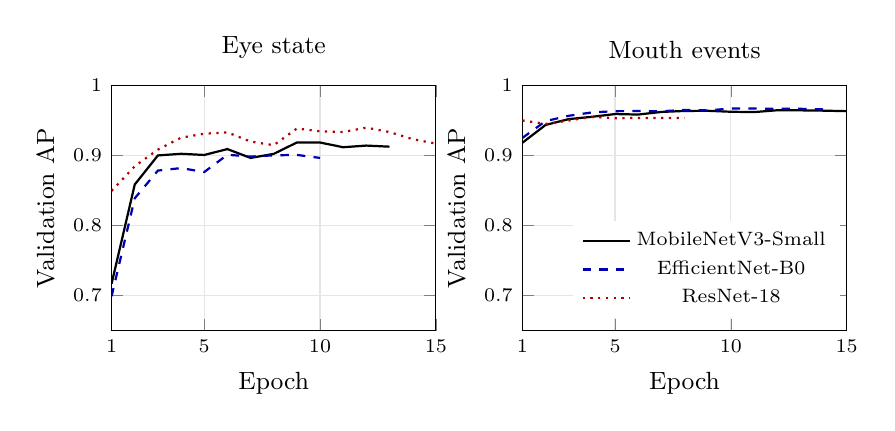
\begin{tikzpicture}
\begin{groupplot}[group style={group size=2 by 1,horizontal sep=11mm},width=0.47\textwidth,height=4.7cm,scale only axis=false,xlabel={Epoch},ylabel={Validation AP},xmin=1,xmax=15,ymin=0.65,ymax=1,xtick={1,5,10,15},ytick={0.7,0.8,0.9,1},grid=major,grid style={gray!20},tick label style={font=\scriptsize},label style={font=\small},title style={font=\small},legend style={font=\scriptsize,draw=none,at={(0.98,0.05)},anchor=south east},legend columns=1]
\nextgroupplot[title={Eye state}]
\addplot[black,solid,thick] coordinates {(1,0.7170823365807807) (2,0.8583798957722779) (3,0.8998018484876057) (4,0.9021416817680594) (5,0.9004690785476326) (6,0.9088466873282006) (7,0.8962386932081879) (8,0.902010275834801) (9,0.9182391716620932) (10,0.9182076191762785) (11,0.9114878864211694) (12,0.9138427537464863) (13,0.9122953458570492)};
\addplot[blue!70!black,dashed,thick] coordinates {(1,0.6990446238519893) (2,0.8387318580509724) (3,0.8782332239061222) (4,0.8817478723934392) (5,0.8761433919378941) (6,0.9007678555505568) (7,0.898191847371079) (8,0.8999434682360983) (9,0.9005490936510667) (10,0.8962519539071014)};
\addplot[red!70!black,dotted,thick] coordinates {(1,0.8492886796438827) (2,0.8843970357077421) (3,0.9081476042776259) (4,0.9250955923703065) (5,0.9307601706671971) (6,0.9327469362460601) (7,0.9195548299585894) (8,0.9144016557596645) (9,0.9381641253507574) (10,0.9342444124540603) (11,0.9332706741437716) (12,0.9393502121473437) (13,0.9331355982545702) (14,0.9230112156779031) (15,0.9166670207012797)};
\nextgroupplot[title={Mouth events}]
\addplot[black,solid,thick] coordinates {(1,0.9179011156017488) (2,0.9432289773142976) (3,0.951572367610097) (4,0.9548779223418228) (5,0.958782357563443) (6,0.9580832685440196) (7,0.961787671540514) (8,0.9631957589187498) (9,0.9634104745160044) (10,0.9620564635274858) (11,0.9615508603785133) (12,0.9642046627053547) (13,0.9640537281666176) (14,0.9636285232389149) (15,0.9628973437541687)};
\addlegendentry{MobileNetV3-Small}
\addplot[blue!70!black,dashed,thick] coordinates {(1,0.924784287093237) (2,0.9487469253128499) (3,0.9563254655018755) (4,0.961091819566926) (5,0.9628896025127857) (6,0.9631384162127589) (7,0.9627951517770098) (8,0.9645969603159622) (9,0.9639903433053498) (10,0.9666281546769246) (11,0.9665866692566336) (12,0.9663445763606404) (13,0.9662567939477128) (14,0.9654381651342584)};
\addlegendentry{EfficientNet-B0}
\addplot[red!70!black,dotted,thick] coordinates {(1,0.9496311783905848) (2,0.9446989342406021) (3,0.9495645348867919) (4,0.954726705291404) (5,0.9528858151069993) (6,0.9530771857358818) (7,0.9532691184213046) (8,0.9532137090411532)};
\addlegendentry{ResNet-18}
\end{groupplot}
\end{tikzpicture}

\caption{Validation AP histories for the eye task and macro AP for the mouth task, reproduced from saved training CSV files. Curves have different lengths because training can stop early.}\label{fig:training}
\end{figure}

\begin{table}[htbp]
\caption{Task-specific resource counts. Parameters and MACs are shown as eye / mouth; storage covers the pair's FP32 parameters only.}\label{tab:resources}
\begin{tabularx}{\textwidth}{@{}Yrrr@{}}
\toprule
Architecture & Parameters (M) & MACs (M) & Pair MiB \\
\midrule
MobileNetV3-Small & 1.519 / 1.521 & 21.05 / 17.72 & 11.60 \\
EfficientNet-B0 & 4.009 / 4.011 & 141.66 / 118.15 & 30.59 \\
ResNet-18 & 11.177 / 11.178 & 666.21 / 555.17 & 85.28 \\
\bottomrule
\end{tabularx}
\end{table}

The MobileNet eye model uses approximately 7.36 times fewer parameters than ResNet-18, with a balanced-accuracy difference of 0.95 percentage points. The mouth difference is 1.15 percentage points. The resource counts in Table~\ref{tab:resources} support the choice of MobileNet for the current CPU prototype; they do not establish a matched latency or energy advantage because all three models were not timed under the same complete application workload. The live service loads two PyTorch \texttt{.pth} checkpoints. ONNX exports are available, but an ONNX file size is not the application's peak memory use.

A saved microbenchmark on an Apple M4 used PyTorch 2.13.0, four CPU threads, 20 warm-up calls and 100 measured calls. For the deployed eye-and-mouth pair plus normalisation on synthetic image crops, the recorded median was 94.31 ms and the 95th percentile was 99.66 ms. Face extraction, JPEG handling, HTTP transport and the browser were excluded. These measurements therefore describe classifier processing rather than end-to-end camera response time.

\subsection{Interface behaviour}
The interface provides an entry page, model comparison, camera monitoring, telemetry controls, evidence bars and intervention actions. It exposes current and next alert stages so that an examiner can connect a displayed decision to its thresholds. Speed and driving duration are manually controlled; the initial speed is zero and inference remains idle until it is increased. A reset clears session evidence.

Figures~\ref{fig:intervention} and \ref{fig:route} show saved application screenshots. The intervention image was created using the examiner's demonstration control. Its warning is independent of a detected camera event. The route image displays the accepted hardcoded destination and path. These figures document interface behaviour, not live detection accuracy or an actual navigation service.

\begin{figure}[htbp]
\centering
\includegraphics[width=\textwidth]{figures/ui_intervention.jpg}
\caption{Examiner-triggered microsleep intervention with voice and rest actions. This saved screenshot does not demonstrate camera-based detection.}\label{fig:intervention}
\end{figure}
\begin{figure}[htbp]
\centering
\includegraphics[width=\textwidth]{figures/ui_reroute.jpg}
\caption{Accepted demonstration route to a predefined rest plaza. The path, distance and travel time are fixed interface values.}\label{fig:route}
\end{figure}

\subsection{Temporal verification and integration finding}
Eight temporal-engine unit tests passed during this report's verification. They cover temporal accumulation, sensor validity, yawn counting, timestamp checks and context sensitivity. A separate deterministic check exposed an integration problem that those tests do not cover: the browser schedules observations at 700 ms, but sustained closure requires consecutive observations no more than 500 ms apart.

Table~\ref{tab:timing} reports a controlled engine reproduction using closed-eye probability 0.9, no yawns, a valid face, speed 100 km/h and continuous-drive duration 120 minutes. At 100 ms spacing, closure accumulates. At 700 ms spacing, each sample restarts closure tracking, so its reported duration remains zero. PERCLOS can still trigger after sufficient observation because the engine records 0.5 s of each 0.7 s interval, giving approximately 71.43\% coverage. At 1.4 s spacing, coverage falls to 35.71\%, below the PERCLOS readiness requirement.

\begin{table}[htbp]
\caption{Deterministic observation-cadence checks. These are engine inputs, not recorded driver events.}\label{tab:timing}
\begin{tabularx}{\textwidth}{@{}rrrrY@{}}
\toprule
Interval & Time & Closure & Coverage & Outcome \\
\midrule
0.1 s & 5.0 s & 5.0 s & 100\% & Critical from sustained closure \\
0.7 s & 4.9 s & 0.0 s & 71.43\% & No alert \\
0.7 s & 21.0 s & 0.0 s & 71.43\% & Critical from PERCLOS \\
1.4 s & 21.0 s & 0.0 s & 35.71\% & No alert \\
\bottomrule
\end{tabularx}
\end{table}

The current sustained-closure pathway therefore cannot be considered dependable at the nominal browser cadence. The capture schedule, timestamp semantics and continuity allowance must be reconciled and tested together. Increasing the permitted gap without checking dropped frames could bridge unobserved periods and create a different error. Appropriate verification should measure actual frame-arrival intervals, processing delays, missed requests and detection delay using annotated sequences.

\FloatBarrier
\section{Limitations and Future Work}\label{sec:limits}
The most immediate limitation is the temporal integration mismatch. Correcting it should precede claims of reliable microsleep alerts. The current closed-eye and yawn labels are visual proxies for fatigue; no physiological confirmation of microsleep or driver impairment is provided. Manual demonstration buttons cannot validate this detection pathway.

The dataset evidence is also provisional. Weak labels can reproduce errors from the labelling rules, and correlated crops can make frame counts overstate the effective amount of independent information. Participant-disjoint splits are useful, but they do not establish independent ground truth or statistical significance. The reported results come from one saved training run per architecture and task. Future work should add independently annotated test sequences, participant-level confidence intervals, repeated runs and cross-dataset transfer tests.

Operating conditions require separate evaluation. Changes in lighting, face pose, sunglasses, occlusion, blur and camera placement can affect extraction and classification. The approximate OpenCV fallback should be evaluated independently from the landmark pathway. The current processing pipeline should not be described as validated denoising or as robust to these conditions merely because it contains augmentation and compact network blocks.

The context policy uses simulated speed and drive duration and has no measured benefit over a fixed policy. An appropriate experiment would hold visual evidence constant and compare fixed thresholds, confidence-adaptive windows and the current context adaptation. Detection delay, missed events, false alarms per hour and alert frequency should be measured on the same sequences. Yawn handling under long observation gaps, the 12 s intervention throttle and driver response to repeated speech also require evaluation.

Finally, deployment needs end-to-end latency, memory and energy measurements on target hardware. Vehicle telemetry and real routing would require additional integration and testing. The local prototype does not establish production privacy, security, availability or automotive safety certification. These limitations define the next engineering steps rather than diminishing the value of the current component comparison.

\section{Conclusion}
DriveAlert AI combines two compact visual classifiers, a deterministic fatigue engine and a browser intervention interface. In the saved participant-disjoint crop evaluation, MobileNetV3-Small achieved 96.93\% eye and 94.41\% mouth balanced accuracy against provisional weak labels. ResNet-18 produced higher classification scores at a larger computational cost. The current implementation demonstrates local model integration, inspectable alert rules and simulated rest intervention. A confirmed timing mismatch limits sustained-closure detection in the browser, and the benefit of context adaptation has not been measured. Correcting temporal integration and evaluating independently labelled driver sequences are the next requirements for a defensible claim about complete-system fatigue detection.

\backmatter
\bmhead{Project roles}
Group 13 presents this work for 21CSC302 Deep Learning / Capstone Project under the guidance of Dr. Bagyammal T, Professor, Department of Computer Science and Engineering. The review presentation assigns MobileNetV3-Small deployment to Krishnan S (CB.SC.U4CSE23628), EfficientNet-B0 comparison to Adwaith Raveendran (CB.SC.U4CSE23603), and ResNet-18 comparison to Eric Febin (CB.SC.U4CSE23717).

\bmhead{Code and data availability}
Project code and model-evaluation artefacts are maintained at \url{https://github.com/krishnans4132/DriveAI}. Raw dataset videos and extracted image datasets are not distributed with the repository; access is through the original providers. The report describes the local project state inspected on 28 September 2026. Source-level evidence is summarised in Appendix~\ref{app:reproducibility}.

\begin{appendices}
\section{Reproducibility and Evidence}\label{app:reproducibility}
The application entry points are \texttt{backend/app.py} for the local service and \texttt{src/components/DashcamView.jsx} for camera capture. Model inference is in \texttt{backend/model\_runtime.py}; crop extraction is in \texttt{backend/vision.py}; the temporal rules are in \texttt{backend/fatigue\_engine.py}. The simulator, telemetry panel and intervention components implement the visible workflow. These files are the primary evidence for current behaviour.

The deployed metrics, thresholds, checkpoints and histories are under \texttt{ml/models/eye\_v3/} and \texttt{ml/models/mouth\_v1/}. EfficientNet and ResNet comparison reports are under \texttt{ml/results/}. The architecture notebooks are under \texttt{ml/notebooks/}. Saved parameter counts and the synthetic-crop timing measurement are in \texttt{presentation\_assets/evidence.json}. The report's metric tables and graphs use these stored results; the models were not retrained for report preparation.

To reproduce the demonstration, install the frontend dependencies from the package manifest and the Python dependencies from \texttt{backend/requirements.txt}. Start the backend using \texttt{python backend/app.py}, then the interface using \texttt{npm run dev}. Allow webcam access and enable voice alerts through the interface. Record real request intervals before interpreting sustained-closure behaviour. The actual training workflow is contained in the notebooks; \texttt{backend/train.py} is a demonstration placeholder.

For the temporal checks, run \texttt{python -m unittest discover -s backend/tests}. Model-runtime tests additionally require the trained checkpoints and the documented numerical and machine-learning dependencies. The eight fresh passing tests reported here concern the temporal engine; no fresh full-suite or physical-camera pass is claimed.
\end{appendices}

\begingroup
\interlinepenalty=10000
\bibliography{references}
\endgroup
\end{document}
